\documentclass[serif, xcolor={svgnames, table}, usepdftitle=false]{beamer}

% Beamer
\usetheme{CambridgeUS}
\usecolortheme{beaver}

% Fonts
\usepackage{fontspec}

% Languages and bibliographies
\usepackage{polyglossia}
\usepackage{csquotes}
\usepackage[hyperref, backref, backend=biber]{biblatex}

% Mathematics
\usepackage{mathtools}
\usepackage[math-style=TeX, bold-style=upright]{unicode-math}
\usepackage{stmaryrd}

% Pseudocode
\usepackage{algorithm}
\usepackage{algpseudocode}
\usepackage{varwidth}

% Microtype
\usepackage{microtype}

% Graphics and captioning
\usepackage{graphicx}
\usepackage{caption}
\usepackage{subcaption}

% Tables
\usepackage{booktabs}

% Numbers
\usepackage{siunitx}
\usepackage{nth}

%
% Package setup
%

\setmainlanguage{english}
\setmathfont{Latin Modern Math}
\mathtoolsset{mathic=true}
\sisetup{%
  detect-all,
  detect-display-math,
  binary-units
}

\addbibresource{Bibliography.bib}

\hypersetup{%
  unicode,
  pdfinfo={%
    Title={Introduction to Word Vectors},
    Subject={Deep Learning},
    Author={Dario Gjorgjevski},
    Keywords={Word Vectors, Deep Learning, Machine Learning, Neural Network,
      Language Model, Distributional Semantics}
  },
  linkcolor=MediumBlue,
  urlcolor=DarkCyan,
  citecolor=ForestGreen
}

\renewcommand*{\vec}{\symbf}
\newcommand*{\mat}{\symbf}
\DeclarePairedDelimiter\abs{\lvert}{\rvert}
\DeclarePairedDelimiter\norm{\lVert}{\rVert}

\newtheorem{assumption}{Assumption}

\graphicspath{{Figures/}}

%
% Title
%

\title{Introduction to Word Vectors}
\subtitle{Learning Word Vectors Using \texttt{word2vec} and Reasoning With Them}
\author[Dario Gjorgjevski]{%
  Dario Gjorgjevski\inst{1}\\%
  \href{mailto:gjorgjevski.dario@students.finki.ukim.mk}%
  {\texttt{gjorgjevski.dario@students.finki.ukim.mk}}
}
\institute[FCSE]{%
  \inst{1}Faculty of Computer Science and Engineering\\%
  Ss.\ Cyril and Methodius University in Skopje
}
\date{\today}

%
% Logo
%

% \logo{
\includegraphics[height=0.66cm]{Logo.png}}

%
% Table of contents
%

\AtBeginSection[]{%
  \begin{frame}{Contents}
    \tableofcontents[currentsection, hideothersubsections]
  \end{frame}
}


\begin{document}

%
% Custom commands
%

\newcommand{\wi}{\ensuremath{w^{\mathrm{(in)}}}}
\newcommand{\wo}{\ensuremath{w^{\mathrm{(out)}}}}
\newcommand{\wn}{\ensuremath{w^{\mathrm{(neg)}}}}
\newcommand{\Wn}{\ensuremath{\mathcal{W}^{\mathrm{(neg)}}}}

%
% Document
%

\begin{frame}
  \titlepage
\end{frame}

\section{Motivation}

\subsection{Language Models}

\begin{frame}{What is a language model?}
  \begin{definition}[Language model]
    A \emph{language model} is a probability distribution over word sequences.
    More formally, given a word sequence \(w_1, \ldots, w_m\), the language
    model assigns a probability
    \[
      p(w_1, \ldots, w_m)
    \]
    to the whole sequence.
  \end{definition}

  Until recently, the most widely used language model was the \emph{\(n\)-gram
    model}, which assumes an \(n\)th order Markov property.
\end{frame}

\begin{frame}{\(n\)-gram model}{Concept}
  In an \(n\)-gram model, the probability \(p(w_1, \ldots, w_m)\) is
  approximated as
  \begin{align*}
    p(w_1, \ldots, w_m) &= \prod\limits_{i = 1}^{m} p(w_i \mid w_1, \ldots,
                          w_{i - 1}) \\
                        & \approx \prod\limits_{i = 1}^{m} p(w_i \mid w_{i - (n - 1)},
                          \ldots, w_{i - 1})\text{.}
  \end{align*}
  \begin{itemize}
  \item The conditional probabilities can be calculated by counting; however,
  \item \emph{Smoothing} is required for unseen \(n\)-grams.
  \end{itemize}
\end{frame}

\begin{frame}{\(n\)-gram model}{Issues}
  \begin{itemize}
  \item As the \(n\)-gram model is trained on larger and larger texts, the
    vocabulary size increases as \(K n^{\beta}\) with \(10 \le K \le 100\) and
    \(0.4 \le \beta \le 0.6\) (\emph{Heaps' law}).
  \item As the vocabulary size increases, the number of possible sequences of
    words increases exponentially \(\implies\) data sparsity problems.
  \item Ultimately, we are not sure how a word is to be even represented, and
    the \(n\)-gram model does not provide us with any clues toward that
    direction.
  \end{itemize}
\end{frame}

\subsection{Word Vectors}

\begin{frame}{Localist representations}
  These representations are also called \emph{one-hot}.  They dedicate one unit
  to each word.
  \begin{itemize}
  \item Easy to understand.
  \item Easy to code by hand.
    \begin{itemize}
    \item Have been used as inputs to machine learning algorithms, especially
      neural networks.
    \end{itemize}
  \item Easy to learn.
    \begin{itemize}
    \item It is what mixture models (e.g.\ hidden Markov models) do.
    \end{itemize}
  \item Easy to associate with other representations or responses.
  \end{itemize}

  \alert{However}, they are terribly inefficient when the data has componential
  structure---and language does.
\end{frame}

\begin{frame}{Localist representations}{Issues}
  In vector space terms, these are vectors with one \(1\) and lots of \(0\)s:
  \[
    \begin{bmatrix}
      \ldots & 0 & 0 & 1 & 0 & 0 & \ldots
    \end{bmatrix}\text{.}
  \]
  \begin{itemize}
  \item These vectors are \emph{extremely} sparse.
  \item They do not encode encode similarities whatsoever, i.e.
    \[
      \forall i \ne j\ldotp \vec{w}_i \wedge \vec{w}_j = \vec{0}
    \]
    even if \(\vec{w}_i\) and \(\vec{w}_j\) are inherently similar.
  \end{itemize}
\end{frame}

\begin{frame}{Distributional representations}
  A lot of information can be obtained by representing a word by means of its neighbors.
  \begin{displayquote}
    You shall know a word by the company it keeps.\par\hfill--- J.\ R.\ Firth
  \end{displayquote}
  How do we learn distributional representations?
  \begin{itemize}
  \item Directly, using co-occurrence matrices; or
  \item As a side-effect by training neural networks to predict either the word
    given its context, or the context given a word (\emph{continuous space
      language models}).
  \end{itemize}
\end{frame}

\section{Learning Word Vectors}

\subsection{Learning Context by Counting}

\begin{frame}{Co-occurrence matrices}
  \begin{definition}[Co-occurrence matrix]
    Let \(\{w_1, w_2, \ldots, w_V\}\) be the vocabulary.  A \emph{co-occurrence
      matrix} is a \(V \times V\) matrix which counts how many times a pair of
    words \((w_i, w_j)\) appear together in some context.
  \end{definition}
  \begin{itemize}
  \item Very straightforward solution.
  \item Can learn either:
    \begin{itemize}
    \item General topics by considering full documents as contexts; or
    \item Syntactic and semantic information by using a window context.
    \end{itemize}
  \end{itemize}

  The context is usually taken to be a window of size \(k\).
\end{frame}

\begin{frame}{Co-occurrence matrices}{Issues}
  \begin{itemize}
  \item Dimension increases quadratically with \(V\) \(\implies\) huge storage
    requirements, sparsity issues in classifiers.
  \item Models are less robust because of sparsity issues.
  \item Low-dimensional vectors can be obtained by SVD.  Unfortunately,
    computing the SVD of an \(m \times n\) matrix requires
    \(\mathcal{O}(m^2 n)\) operations:
    \begin{itemize}
    \item Computationally infeasible for millions of words.
    \item Hard to incorporate new data.
    \end{itemize}
  \end{itemize}

  \structure{Where do we go from here?}  We do not count anymore; instead, we
  directly learn low-dimensional dense vectors by neural network prediction.
\end{frame}

\subsection{Learning Context by Prediction}

\begin{frame}{What to predict?}
  Two models have received most attention in literature:
  \begin{itemize}
  \item \emph{Continuous bag-of-words} (CBOW) model, which predicts target words
    (e.g.\ ``mat'') from source context words (e.g.\ ``the cat sits on the'');
    and
  \item \emph{Skip-gram} model, which predicts source context words from the
    target words.
  \end{itemize}

  CBOW smoothes over a lot of the distributional information by treating an
  entire context as a single observation, while skip-gram treats every
  context--target pair as a new observation.
\end{frame}

\begin{frame}{Continuous bag-of-words model}
  \begin{figure}
    \centering
    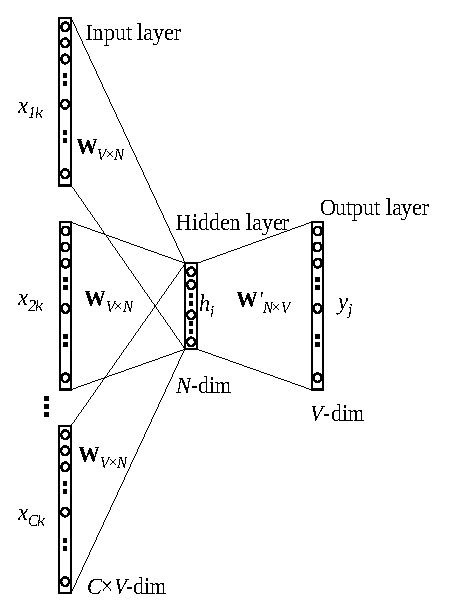
\includegraphics[width=.4\textwidth]{CBOW.pdf}
    \caption{CBOW model with \(C\) words in the context.}
  \end{figure}
\end{frame}

\begin{frame}{Continuous bag-of-words model}{Mathematical definition}
  \begin{itemize}
  \item The input consists of one-hot encoded words,
    \(\vec{x}_1, \ldots, \vec{x}_C\).
  \item The input \(\to\) hidden and hidden \(\to\) output weights are
    represented by \(\mat{W}\) and \(\mat{W}'\) respectively.  The rows of
    \(\mat{W}\) (the \(\vec{v}_w\)'s) and the columns of \(\mat{W}'\) (the
    \(\vec{v}'_w\)'s), give the \alert{\(N\)-dimensional input} and
    \alert{output representations} of a word \(w\).
  \item The hidden layer is \emph{linear} and computes an average
    \[
      \vec{h} \coloneqq \frac{\left(\sum\nolimits_{c = 1}^{C} \vec{x}_c\right)
        \mat{W}}{C} = \frac{\sum\nolimits_{c = 1}^{C}
        \vec{v}_{\wi_c}}{C}\text{.}
    \]
  \item The output layer is a softmax panel outputting a multinomial
    distribution over the vocabulary.
  \end{itemize}
\end{frame}

\begin{frame}{Continuous bag-of-words model}{Update equations}
  As usual with softmax, the cross-entropy loss function is used,
  \begin{equation}\label{eq:cbow-cross-entropy-loss}
    \begin{aligned}
      E &\coloneqq -\log p(\wo \mid \wi_1, \ldots, \wi_C) \\
      &= -\vec{v}_{\wo}^{\prime\intercal} \vec{h} + \log \sum\limits_{v = 1}^{V}
      \exp(\vec{v}_{w_v}^{\prime\intercal} \vec{h})\text{.}
    \end{aligned}
  \end{equation}

  By taking the corresponding derivatives of~\eqref{eq:cbow-cross-entropy-loss},
  we arrive at the update equations:
  \begin{equation}\label{eq:cbow-weight-update}
    \begin{aligned}
      \vec{v}'_{w_v}&\coloneqq \vec{v}'_{w_v} - \eta e_v \vec{h} && (\forall 1 \le v \le V) \\
      \vec{v}_{\wi_c} &\coloneqq \vec{v}_{\wi_c} - \frac{\eta}{C} \frac{\partial
        E}{\partial \vec{h}} && (\forall 1 \le c \le C)\text{.}
    \end{aligned}
  \end{equation}
\end{frame}

\begin{frame}{Continuous bag-of-words model}{Understanding the update equations}
  The derivatives in~\eqref{eq:cbow-weight-update} can be computed using
  backpropagation:
  \begin{align*}
    e_v &= \text{prediction error for word }v\text{,} \\
    \frac{\partial E}{\partial h_i} &= \sum\limits_{v = 1}^{V} e_v w'_{i v}\text{.}
  \end{align*}
  Intuitively,
  \begin{itemize}
  \item If we overestimate (resp.\ underestimate) the probability for word
    \(w_v\), we subtract from (resp.\ add to) \(\vec{v}'_{\wo}\) a portion of
    the input \(\implies\) \(\vec{v}'_{\wo}\) becomes closer to the averaged
    input vectors.
  \item Since \(\partial E / {\partial \vec{h}}\) is the sum of all output
    vectors weighted by their prediction errors, \eqref{eq:cbow-weight-update}
    can be seen as distributing a portion of every output vector to each of the
    \(C\) input vectors.
  \end{itemize}
\end{frame}

\begin{frame}{Skip-gram model}
  \begin{figure}
    \centering
    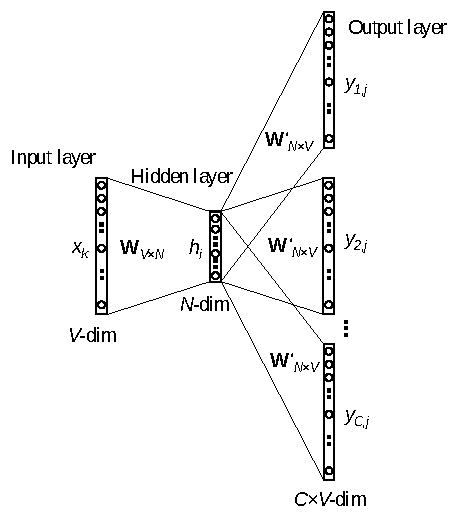
\includegraphics[width=.4\textwidth]{Skip-Gram.pdf}
    \caption{Skip-gram model for predicting \(C\) context words.}
  \end{figure}
\end{frame}

\begin{frame}{Skip-gram model}{Mathematical definition}
  \begin{itemize}
  \item The input consists of a one-hot encoded word, \(\vec{x}\), with
    \(x_k = 1\) and \(x_i = 0\) for all \(i \ne k\).
  \item The weights encode the same information as in the CBOW model.
  \item The hidden layer simply copies the row of the matrix \(\mat{W}\)
    associated with the input word \(\wi\):
    \[
      \vec{h} = \mat{W}_{(k, \cdot)} \eqqcolon \vec{v}_{\wi}\text{.}
    \]
  \item The output layer consists of \(C\) softmax panels, and outputs \(C\)
    multinomial distributions over the vocabulary.
  \end{itemize}
\end{frame}

\begin{frame}{Skip-gram model}{Update equations}
  Again, we use the cross-entropy loss function.  Note that care must be taken
  as we are now dealing with \(C\) multinomial distributions rather than just
  one.
  \begin{align*}
    E &\coloneqq -\log p(\wo_1, \ldots, \wo_C \mid \wi) \\
      &= -\sum\limits_{c = 1}^{C} \vec{v}_{\wo_c}^{\prime\intercal} \vec{h} + C \log \sum\limits_{v = 1}^{V}
        \exp(\vec{v}_{w_v}^{\prime\intercal} \vec{h})\text{.}
  \end{align*}

  The equations are identical as in the CBOW model, except the prediction errors
  must be summed across all \(C\) softmax panels.
  \[
    e_v = \sum\limits_{c = 1}^{C}(\text{prediction error of the }c\text{th
      softmax panel for word }v)\text{.}
  \]
\end{frame}

\begin{frame}{Issues with the CBOW and skip-gram models}
  \begin{itemize}
  \item Both models are very similar in their nature and have a same intuitive
    interpretation.
  \item Due to the smoothing, CBOW is recommended for small datasets; while
    skip-gram is able to learn better representations give sufficient data
    (``there is no better regulizer than a large dataset'').
  \item Unfortunately, both are very hard to train.
  \end{itemize}

  We tried to avoid the vast size of the vocabulary as hard as possible,
  however, \eqref{eq:cbow-weight-update} performs \(\mathcal{O}(V)\) weight
  updates for both the CBOW and skip-gram models.  To ameliorate this and make
  learning practical, we will look at
  \begin{itemize}
  \item hierarchical softmax; and
  \item negative sampling.
  \end{itemize}
\end{frame}

\subsection{Making Learning by Prediction Practical}

\begin{frame}{Hierarchical softmax}
  The hierarchical softmax uses a binary tree to represent the vocabulary.
  There are \(V\) leaves, one for each word; and \(V - 1\) inner units.
  \begin{figure}
    \centering
    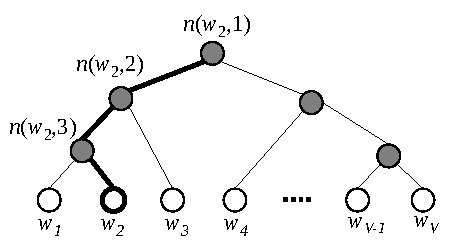
\includegraphics[width=.5\textwidth]{Hierarchical_Softmax.pdf}
    \caption{Example hierarchical softmax with path to \(w_2\).}
  \end{figure}  
\end{frame}

\begin{frame}{Hierarchical softmax}{Details}
  \begin{itemize}
  \item There is no output vector representation---each of the \(V - 1\) inner
    units has an output vector \(\vec{v}_{n(w, j)}\).
  \item The probability of a word being the output word is
    \[
      \Pr(w = \wo) = \prod\limits_{j = 1}^{L(w) - 1} \sigma(\llbracket n(w, j +
      1) = \operatorname{left}(n(w, j))\rrbracket
      \vec{v}^{\prime\intercal}_{n(w, j)} \vec{h})\text{,}
    \]
    where \(L(w)\) is the length of the path to word \(w\),
    \(\operatorname{left}(n(w, j))\) is the left child of the inner unit
    \(n(w, j)\), \(\sigma\) is the sigmoid function, and
    \[
      \llbracket p \rrbracket =
      \begin{cases}
        1 & \text{if }p\text{ is true}\\
        -1 & \text{otherwise.}
      \end{cases}
    \]
  \end{itemize}
\end{frame}

\begin{frame}{Hierarchical softmax}{Update equations}
  By backtracing the path from the leaves to the root, one obtains the update
  equations for the inner nodes
  \[
    \vec{v}'_{n(w, j)} \coloneqq \vec{v}'_{n(w, j)} - \eta \left(
      \sigma(\vec{v}^{\prime\intercal}_{n(w, j)} \vec{h}) - t_{n(w, j)} \right)
    \vec{h} \quad (\forall 1 \le j \le L(w) - 1)\text{,}
  \]
  where \(t_{n(w, j)}\) denotes the ``ground truth'' at level \(j\) (``left'' or
  ``right'').

  The derivative of the error with respect to the hidden layer can be found as
  \[
    \frac{\partial E}{\partial \vec{h}} = \sum\limits_{j = 1}^{L(w) - 1}
    \left(\sigma(\vec{v}^{\prime\intercal}_{n(w, j)} \vec{h}) - t_j\right)
    \vec{v}'_{n(w, j)}\text{.}
  \]
\end{frame}

\begin{frame}{Hierarchical softmax}{Bottom line}
  \begin{itemize}
  \item Hierarchical softmax can be applied to both the CBOW and skip-gram
    models.
  \item For CBOW, one can plug in the equations directly.  For skip-gram, we
    need to iterate over the entire context we're predicting.
  \item Computational complexity is reduced from \(\mathcal{O}(V)\) to
    \(\mathcal{O}(\log V)\).
  \item Number of parameters remains roughly the same.
  \end{itemize}

  \structure{Can we do even better?}  Turns out, if some heuristic assumptions
  are satisfied, we can.
\end{frame}

\begin{frame}{Negative sampling}
  The idea is very straightforward: instead of updating all output vectors,
  update only a sample of them.

  \begin{assumption}[Negative sampling]
    In order to learn the context, it is enough to update only the output word
    (``ground truth'') along with a few words as negative samples.
  \end{assumption}

  The negative samples are drawn from a noise distribution
  \(p^{\mathrm{(neg)}}(w)\) which is determined empirically.  \texttt{word2vec}
  uses the unigram distribution raised to the power of \(3 / {4}\).
\end{frame}

\begin{frame}{Negative sampling}{Loss function and error derivatives}
  For further heuristics, negative sampling does not use a loss function that
  produces a well-defined posterior multinomial distribution.
  \[
    E = -\log \sigma(\vec{v}^{\prime\intercal}_{\wo} \vec{h}) - \sum_{\wn \in
      \Wn} \log \sigma(-\vec{v}^{\prime\intercal}_{\wn} \vec{h})\text{,}
  \]
  where \(\Wn\) is a set of negative samples.  This results in updates very
  similar to the hierarchical softmax.  Letting
  \(\mathcal{W} \coloneqq \{\wo\} \cup \Wn\),
  \begin{align*}
    \vec{v}'_{w_j} &\coloneqq \vec{v}'_{w_j} - \eta \left(\sigma(\vec{v}^{\prime\intercal}_{w_j} \vec{h})
                     - t_j\right) \vec{h} \quad (\forall w_j \in \mathcal{W}) \\
    \frac{\partial E}{\partial \vec{h}}
                   &=
                     \sum\limits_{w_j \in \mathcal{W}} \frac{\partial E}{\partial
                     \vec{v}^{\prime\intercal}_{w_j} \vec{h}} \frac{\partial
                     \vec{v}^{\prime\intercal}_{w_j} \vec{h}}{\partial \vec{h}}
                   = \sum\limits_{w_j \in \mathcal{W}}
                     \left(\sigma(\vec{v}^{\prime\intercal}_{w_j} \vec{h}) - t_j\right) \vec{v}'_{w_j}\text{,}
  \end{align*}
  where \(t_j \coloneqq \mathbb{1}\{w_j = \wo\}\).
\end{frame}

\begin{frame}{Further improvements}{Subsampling}
  In order to counter the imbalance between rare and frequent words,
  \texttt{word2vec} uses subsampling.  Namely, each word in the training set is
  discarded with probability
  \[
    1 - \sqrt{\frac{d}{f(w_j)}}\text{,}
  \]
  where \(f(w_j)\) is the frequency of the word \(w_j\) and \(d\) is the discard
  threshold, typically around \num{e-5}.
\end{frame}

\section{Reasoning With Word Vectors}

\begin{frame}{Country--capital city relationships}
  \begin{figure}
    \centering
    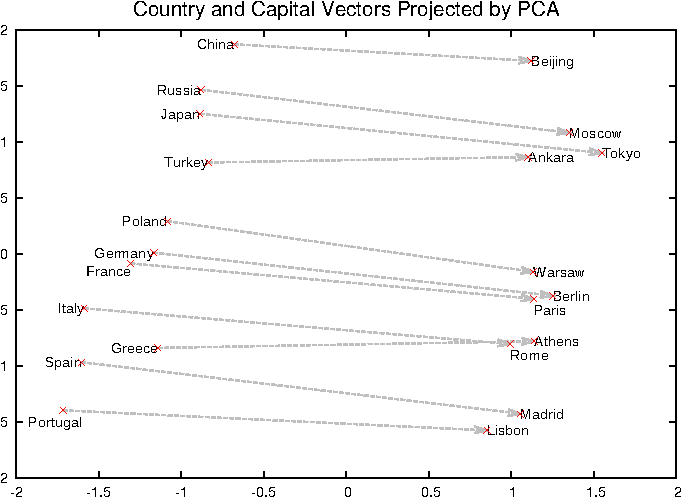
\includegraphics[width=.75\textwidth]{Country--Capital_Vectors.pdf}
    \caption{Country--capital city relationships projected with PCA.}
  \end{figure}  
\end{frame}

\begin{frame}{Phrase representations}
  The aforementioned models are not restricted only to words---they can use
  phrases and other constructs just as well.
  \begin{table}
    \centering
    \caption{Phrase analogy with \num{e-5} subsampling.}
    \begin{tabular}{c c c}
      \toprule
      Phrase & NEG & HS \\
      \midrule
      Vasco de Gamma & Lingsugur & Italian explorer \\
      Lake Baikal & Great Rift Valley & Aral Sea \\
      Alan Bean & Rebbeca Naomi & moonwalker \\
      Ionian Sea & Ruegen & Ionian Islands \\
      chess master & chess grandmaster & Garry Kasparov \\
      \bottomrule
    \end{tabular}
  \end{table}
\end{frame}

\begin{frame}{Additive compositionality}
  Interestingly, element-wise addition yields meaningful combinations, too.
  This property can be explained by looking at the training objective: the
  vectors are related logarithmically to the probabilities computed by the
  output layer, so the sum of two word vectors is related to the product of the
  two context distributions.
  \begin{table}
    \centering
    \caption{Additive compositionality showing the \num{4} closest vectors.}
    \resizebox{\linewidth}{!}{%
      \begin{tabular}{c c c c c}
        \toprule
        Czech + currency & Vietnam + capital & German + airlines & Russian + river
        & French + actress \\
        \midrule
        Koruna & Hanoi & airline Lufthansa & Moscow & Juliette Binoche \\
        Czech crown & Ho Chi Minh City & carrier Lufthansa & Volga River &
                                                                           Vanessa
                                                                           Paradis
        \\
        Polish zolty & Viet Nam & flag carrier Lufthansa & upriver & Charlotte
                                                                     Gainsbourg
        \\
        CTK & Vietnamese & Lufthansa & Russia & Cecile De \\
        \bottomrule
      \end{tabular}
    }
  \end{table}
\end{frame}

\end{document}

%%% Local Variables:
%%% mode: latex
%%% fill-column: 80
%%% TeX-command-extra-options: "-shell-escape"
%%% TeX-engine: luatex
%%% TeX-master: t
%%% End: